%% LyX 2.3.3 created this file.  For more info, see http://www.lyx.org/.
%% Do not edit unless you really know what you are doing.
\documentclass[english]{article}
\usepackage[T1]{fontenc}
\usepackage{float}
\usepackage{amsmath}
\usepackage{graphicx}

\usepackage{subcaption}

\makeatletter

%%%%%%%%%%%%%%%%%%%%%%%%%%%%%% LyX specific LaTeX commands.
%% Because html converters don't know tabularnewline
\providecommand{\tabularnewline}{\\}

\makeatother

\usepackage{babel}
\begin{document}
\title{Project 3}
\author{Zachary Taylor,John Dinofrio, Cristian Bueno}
\maketitle

\part*{Project 3}

\textbf{The objective of this project is to use Gaussian Mixture Models and Expectation Maximization techniques to color segment several different colored buoys. The system will learn to segment the colors based on the color distributions  aquired through the two techniques.}
\bigskip

After writing the code to collect the centroids of each buoy, we took an average histogram of each buoy's color distribution. With these distibutions, we were able to create a simple thresholding algorithm basd on the averages and standard deviations. Figure (1) shows the histograms we based our mean and standard deviations on.

\begin{figure}[H]
	\begin{subfigure}{.5\textwidth}
		\centering		
		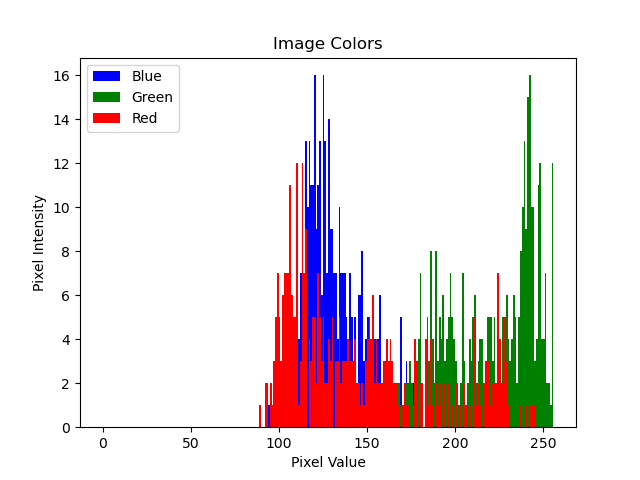
\includegraphics[width=.8\linewidth]{./Figures/green_hist.PNG}  
    	\caption{Histogram of green buoy.}
	\end{subfigure}
	\begin{subfigure}{.5\textwidth}
		\centering
		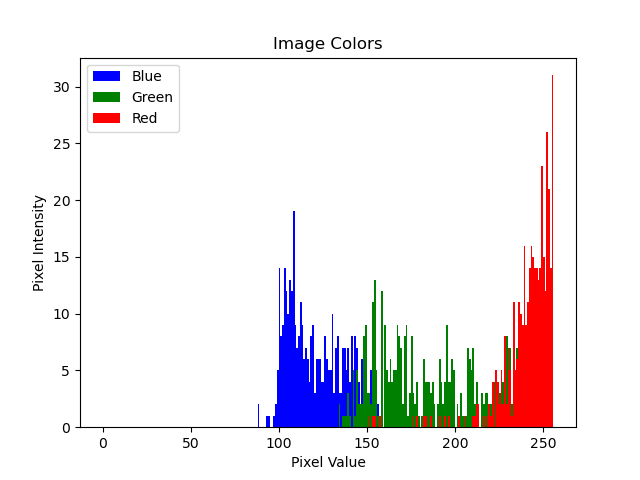
\includegraphics[width=.8\linewidth]{./Figures/red_hist.PNG}
		\caption{Histogram of orange buoy.}
	\end{subfigure}
	\begin{subfigure}{.5\textwidth}
		\centering
		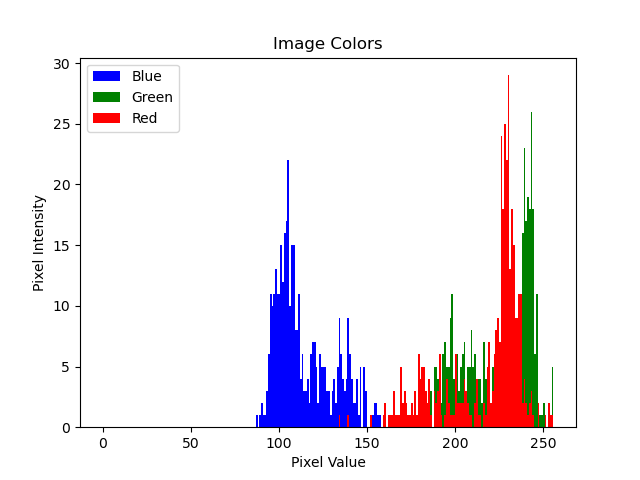
\includegraphics[width=.8\linewidth]{./Figures/yellow_hist.PNG}
		\caption{Histogram of yellow buoy.}
	\end{subfigure}
\end{figure}

Each buoy can be identified by the spike in the mid 200 range on the histograms. For the green buoy, the mean green color was just below 250. For the orange buoy, the mean red color was pretty much at 255. In order to threshold these two, we calculated the 1D Guassian of each histogram. This output gave us the mean and standard deviation of the color channel data. By using the mean and going half a standard deviation up and down, we were able to compute the upper and lower bounds of the threshold. Half a standard deviation was the decided value after multiple tests for thresholding the buoys. Figure (2a-b) shows the thresholded image of the green and orange buoys. For the yellow buoy, we had to use a combination of both the red and green channels. They were both between 230 and 240. We had to apply the 1D Guassian to both channels, threshold them separately using the mean and half of a standard deviation, and then use an AND statement for the two binary outputs. The final threshold can be seen in Figure (2c).

\begin{figure}[H]
	\begin{subfigure}{.5\textwidth}
		\centering		
		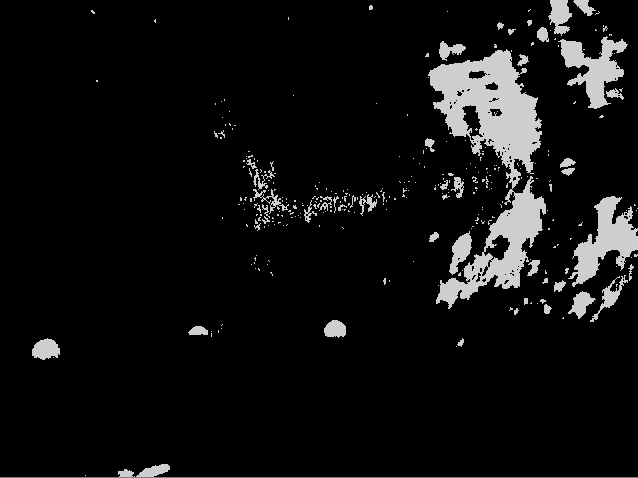
\includegraphics[width=.8\linewidth]{./Figures/green_thresh.PNG}  
    	\caption{Thresholded green buoy.}
	\end{subfigure}
	\begin{subfigure}{.5\textwidth}
		\centering
		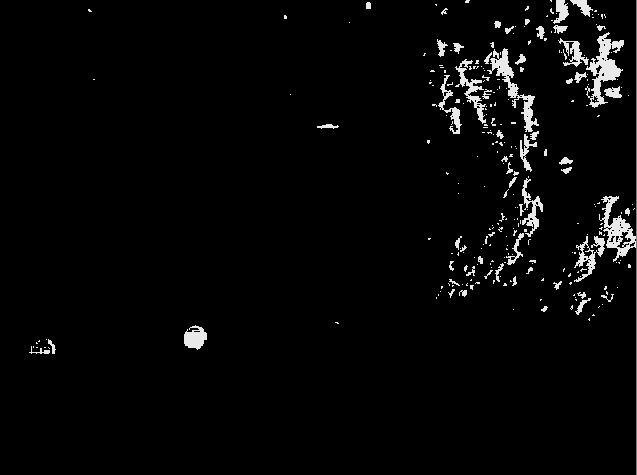
\includegraphics[width=.8\linewidth]{./Figures/red_thresh.PNG}
		\caption{Thresholded orange buoy.}
	\end{subfigure}
	\begin{subfigure}{.5\textwidth}
		\centering
		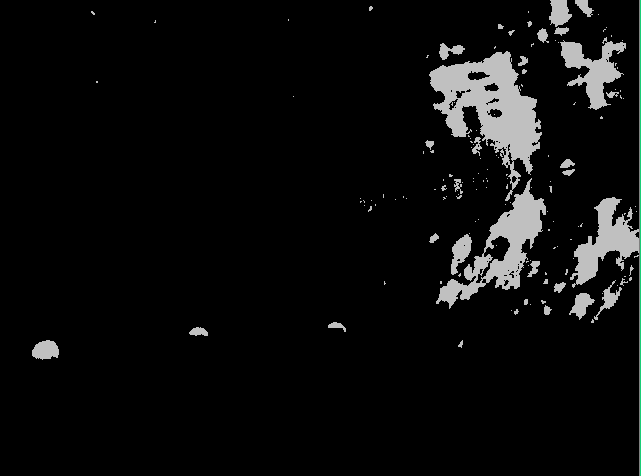
\includegraphics[width=.8\linewidth]{./Figures/yellow_thresh.PNG}
		\caption{Thresholded yellow buoy.}
	\end{subfigure}
\end{figure}




\end{document}
